\documentclass{article}

% Language setting
% Replace `english' with e.g. `spanish' to change the document language
\usepackage[english]{babel}

% Set page size and margins
% Replace `letterpaper' with `a4paper' for UK/EU standard size
\usepackage[letterpaper,top=2cm,bottom=2cm,left=3cm,right=3cm,marginparwidth=1.75cm]{geometry}

% Useful packages
\usepackage{amsmath}
\usepackage{graphicx}
\usepackage[colorlinks=true, allcolors=blue]{hyperref}
\usepackage[colorinlistoftodos,prependcaption,textsize=footnotesize]{todonotes}

\usepackage{natbib} 
\usepackage{booktabs}
\usepackage{textcomp}

\title{PERCUSION’s contribution to ORCESTRA}
\author{PERCUSION crew}

\begin{document}
\maketitle

\begin{abstract}

\end{abstract}


\section{Introduction}
The largest atmospheric field study in history \citep{zhangRelocationGATEPacific2022} was the Global Atmospheric Research Program (GARP) Atlantic Tropical Experiment (GATE) conducted in 1974, which set out to ``explore the mechanism by which solar heat stored in the tropical oceans drives the global circulation of the atmosphere, and to incorporate this mechanism into numerical models'' \citep{kuettnerGeneralDescriptionCentral1974}. 
A key motivation was the recognition that deep convective clouds, while being fundamental to the tropical circulation \citep{riehlHeatBalanceEquatorial1958}, ``slip through the mesh'' of the synoptic-scale observing network \citep{kuettnerGeneralDescriptionCentral1974}.
To collect observations to analyse the effect of deep convective clouds, or smaller-scale weather systems, on the large-scale circulation was, therefore, one of the primary objectives. 
The results revealed, that convective and large-scale processes are not well separated, but rather that complex structures on the mesoscale exist that need to be accounted for \citep{houzejr.ConvectionGATE1981}.
Despite these early insights, the assumption that small and large spatial scales can be cleanly separated has remained a central tenant of our theoretical understanding of tropical climate, as encapsulated by model parameterisations that neglect mesoscale processes governing convective organisation.
While this framework has successfully captured many aspects of anthropogenic climate change, increasing regional discrepancies between observed and simulated changes have renewed attention on mesoscale processes and their coupling to both small- and large-scale processes \citep{shawOtherClimateCrisis2025}.

Exactly fifty years after GATE, the ORCESTRA (Organized Convection and EarthCARE Studies over the Tropical Atlantic) campaign \citep{stevensORCESTRAOrganizedConvection2026} returned to the tropical Atlantic, focusing on mesoscale structures and the processes that govern their formation and evolution.
Taking place from August to September 2024, the campaign combined three research aircraft (\textit{citeBony}), a research vessel (\textit{citeKlocke}) and two observatories \citep{winklerRAPSODIRadiosondeAtmospheric2026}, as well as coordinated measurements with the Earth Cloud Aerosol and Radiation Explorer (EarthCARE) satellite \citep{illingworthEarthCARESatelliteNext2015}, launched less than three months before the start of the campaign. 
Together, these platforms sampled the Atlantic Intertropical Convergence Zone (ITCZ) and adjacent subsiding regions from the ocean floor to the top of the atmosphere. 

ORCESTRA comprised eight sub-campaigns.
This paper summarises the contribution of PERCUSION (Persistent EarthCARE underflight studies of the Intertropical Convergence Zone and organised convection) to ORCESTRA, which utilised the German High Altitude and Long Range Research Aircraft (HALO).
The instrumentation on HALO was designed to resemble that on the EarthCARE satellite, and its calibration and validation were central components of the campaign.
\cite{grossPersistentEarthCAREUnderflight2026} present the contribution of PERCUSION to the calibration and validation of EarthCARE, including research flights in the extratropics.
Here, we focus on the research flights in and around the ITCZ conducted as part of ORCESTRA.
During ORCESTRA, HALO provided vertically resolved ``snapshots” of the mesoscale structure of the atmospheric circulation and thermodynamic state of the ITCZ.
This was enabled by its high-altitude and long-range capabilities, together with its configuration as a cloud observatory \citep{stevensHighAltitudeLongRangeAircraft2019, bonyMeasuringAreaAveragedVertical2019, georgeJOANNEJointDropsonde2021}.

The observations collected during PERCUSION not only provide a benchmark for satellite observations but also for limited-area and global storm-resolving models \citep[e.g.,][]{Klocke2017a, satohGlobalCloudResolvingModels2019, fievetTropicalConvectionStormresolving2026}.
The close link between PERCUSION and both satellite measurements and modelling efforts not only contributes to the calibration and validation of satellite data and models, but also enables us to extrapolate the results from the campaign period and study region to other time periods and locations--a common challenge in targeted field campaigns.

The scientific questions at the heart of the PERCUSION campaign centre on how strongly the “inner life” of the Atlantic ITCZ \citep{windmillerInnerLifeAtlantic2024} shapes its outer life. 
More specifically, we examine how mesoscale structures of clouds, precipitation, surface winds, humidity, and aerosols impact the energy flows, both radiative and through the atmospheric circulation, in the deep tropics.

One pathway through which mesoscale structures affect energy flows is by modifying cloud properties and the associated vertical motion profiles. 
Top-heavy vertical motion profiles, such as those produced by mesoscale convective systems, export energy more efficiently than bottom-heavy profiles, similar to those associated with isolated deep convective cells \citep[e.g.,][]{Houze2004}. 
More recently, it has been suggested that the vertical motion profile of convection also depends on the meridional structure of the ITCZ \citep{masunagaEdgeIntensificationEastern2023}; convection occurring within regions of strong gradients in column water vapor that mark the edges of the deep tropics
\citep{Mapes2018, masunagaMechanismMaintenanceSharp2020}, can differ substantially from convection occurring near its centre. 
These differences may even reverse the sign of the net energy export by the circulation potentially helping to explain regional differences in energy export efficiency found in reanalysis data \citep{backGeographicVariabilityExport2006}. 
Recent work on the doldrums further illustrates the uncertainty surrounding the vertical motion field in the ITCZ \citep{windmillerCalmVariableInner2024}: mesoscale regions of weak surface winds, traditionally interpreted as regions of ascent, may instead be associated with subsiding motion.

Mesoscale structures also influence the thermodynamic properties of the atmosphere. Convective aggregation affects entrainment and detrainment \citep{beckerEstimatingBulkEntrainment2018}, thereby altering the vertical distribution of humidity and temperature \citep[e.g.,][]{singhInfluenceEntrainmentThermal2013}. 
Changes in aggregation are further linked to systematic changes in clouds and radiation. 
More aggregated convection is typically associated with fewer high clouds and a drier troposphere, resulting in increased radiative cooling \citep[e.g.,][]{Tobin2012, bonyObservedModulationTropical2020}. In the tropical Atlantic, radiation is additionally influenced by aerosols transported within the Saharan Air Layer, whose dust and humidity modify radiative heating rates and may affect cloud formation \citep{gutlebenImpactsWaterVapor2019}.

The PERCUSION campaign aimed not only to quantify the effects of mesoscale structures, but also to improve our understanding of the processes that drive them. Tropical convection has long been known to be organised by large-scale disturbances such as equatorial waves \citep[e.g.,][]{kiladisConvectivelyCoupledEquatorial2009} and the Madden-Julian Oscillation \citep{maddenDetection4050Day1971, maddenDescriptionGlobalScaleCirculation1972}. 
In addition to these large-scale drivers, processes acting on smaller scales may also contribute to the organisation of convection.
Idealised simulations show that initially randomly distributed clouds can spontaneously aggregate even in homogeneous environments \citep{Held1993, Bretherton2005}. Depending on the model configuration and the stage of aggregation, a variety of feedbacks have been proposed to drive this behaviour, including convection-humidity feedbacks mediated by detrainment, cloud-radiative feedbacks, and radiatively driven circulations that transport humidity up-gradient \citep[e.g.,][]{Wing2017}.
On yet smaller scales, clouds can trigger the formation of new convection through cold pools, linking successive generations of clouds and organising convection along gust fronts, notably in squall lines \citep{Rotunno1988, Weisman2004}, as well as along the edges of convectively active regions \citep{Nolan2016, windmillerConvectionEdge2019}.
Other processes have also been argued to drive enhanced convection at the edges of the deep tropics \citep{masunagaEdgeIntensificationEastern2023}. Assessing the relative importance of these mechanisms in the real atmosphere remains an open challenge \citep{Bony2015, mullerSpontaneousAggregationConvective2022}.

In order to investigate the impact and drivers of mesoscale structures in the deep tropics, the PERCUSION campaign collected data from the interior and margins of the Atlantic ITCZ, as well as the surrounding subsiding region. This sampling took place in two regions of the tropical Atlantic: first near Sal in the Republic of Cabo Verde in the eastern basin, and later east of Barbados in the western basin. The observations were collected using a systematic sampling strategy designed to characterise the mesoscale structure of the ITCZ rather than to target individual cloud systems. 

A particular focus of PERCUSION was the measurement of quantities central to the tropical energy budget that are rarely accessible observationally. These include vertical profiles of vertical motion derived from dropsonde circles \citep{bonyMeasuringAreaAveragedVertical2019, gloecknerBEACHBarbadosEastern2025}, which constrain the overturning circulation of the tropical atmosphere, and direct observational estimates of convective entrainment, one of the most important yet poorly observed processes shaping convection and its environment \citep{sherwoodSpreadModelClimate2014}. The campaign also collected detailed observations of tropical high clouds--including their microphysical properties and integrated quantities such as ice water path--providing key constraints on the radiative feedback of tropical high clouds, a major uncertainty in climate projections \citep{sherwoodAssessmentEarthClimate2020}.
Many of these measurements rely on retrieval techniques and analysis methods that were further developed during the campaign, and the resulting datasets are being distributed using new approaches designed to facilitate community access and cross-platform analysis.
Together, these observations provide a unique opportunity to link the mesoscale “inner life” of the ITCZ--its clouds, humidity and aerosol structure, and vertical motion--to its influence on the large-scale circulation and radiation budget of the tropical atmosphere.

The remainder of the paper describes the measurement strategy and data (Section 2), presents an overview of the observations (Section 3), and concludes with a discussion of their implications (Section 4).

\section{Data}

This section provides a brief overview of the data collected during PERCUSION, and how this data is now shared. HALO operated in an updated version of the “flying cloud observatory” configuration described by \cite{stevensHighAltitudeLongRangeAircraft2019}. This configuration combines active and passive remote-sensing instruments with in situ measurements from dropsondes, providing a comprehensive view of the atmospheric state, including its thermodynamic and dynamical structure as well as the microphysical properties of clouds and precipitation. While the measurement systems are largely based on those described by \cite{stevensHighAltitudeLongRangeAircraft2019}, they reflect the continued development and enhancement of the instrumentation since that time. The complete configuration used during PERCUSION is shown in Fig.~\ref{fig:instrumentation}.

The core remote-sensing configuration aboard HALO consists of a complementary suite of active and passive instruments designed to characterise the thermodynamic and dynamical structure of the tropical atmosphere, as well as its cloud and aerosol composition and radiative properties. A key component is the HALO Microwave Package (HAMP), which combines a suite of passive microwave radiometers with a cloud radar \citep{mechHAMPMicrowavePackage2014, ewaldCalibration35GHz2019}. The passive radiometers consist of three downward-looking modules with 26 frequencies in different bands between 22.24 and 183.31~GHz $\pm$ 12.5~GHz that sample water vapour and oxygen absorption bands, as well as window channels. These measurements provide information on the different condensate phases of water, as well as on their vertically integrated quantities, such as column water vapour, liquid water path and ice water path. The nadir-pointing microwave cloud and precipitation radar operates at 35.5~GHz (Ka band) and is suitable for penetrating columns with heavy precipitation. It measures radar reflectivity, reflectivity-weighted Doppler velocity, and the linear-depolarization ratio to determine target shape.

Additional active remote sensing is provided by the lidar system WALES (for WAter vapor Lidar Experiment in Space) which was originally developed as an airborne demonstrator for a mission proposal within ESAs Earth Explorer program. WALES operates at four wavelengths near 935~nm to deliver high-resolution profiles of the water vapour mixing ratio below the aircraft using the DIfferential Absorption Lidar (DIAL) technique \citep{wirthAirborneMultiwavelengthWater2009}. Additionally it has backscatter lidar channels at 532- and 1064~nm, where at 532~nm aerosol depolarisation and extinction can be retrieved using the High Spectral Resolution Lidar method (HSRL). At 1064 nm only attenuated backscatter measurements are possible. 

Radiance and irradiance measurements are obtained using the Spectral Modular Airborne Radiation Measurement System (SMART), a suite of passive spectrometers measuring spectral irradiances and radiances within the visible, near-infrared, and shortwave infrared wavelength range (0.3--2.2~\textmu m) \citep{wendischAirborneSpectralAlbedometer2001, wendischACRIDICONCHUVACampaign2016}. The irradiance measurements allow to determine the spectral cloud top albedo, while the radiance measurements can be used to create a cloud flag and to determine microphysical properties, including optical depth and effective droplet radius. 
The spectrometer of the Munich Aerosol Cloud Scanner (specMACS) complements these measurements by providing hyperspectral imaging in the visible/near-infrared (0.4--1.0~\textmu m), and shortwave infrared (1.0--2.5~\textmu m) \citep{ewaldDesignCharacterizationSpecMACS2016} to characterize clouds with respect to their cloud droplet effective radius, cloud droplet size distribution, and cloud optical depth.
%@specMACS team: please add something about the sideways looking cameras
This imaging capability is extended into the thermal infrared by the Video airbornE Longwave Observations within siX channels (VELOX) instrument, which captures high-resolution 2D fields of upward terrestrial radiance across six spectral bands between 7.7 and 12.0~\textmu m, providing information on cloud top brightness temperature, cloud mask/fraction, and cloud top altitude \citep{schaferVELOXNewThermal2022}.
To quantify the cloud radiative effect and the energy budget, HALO utilises the Broadband AirCrAft RaDiometer Instrumentation (BACARDI), which consists of two sets of pyranometers and pyrgeometers mounted to the upper and lower fuselage to measure upward and downward solar(0.3--3 \textmu m) and thermal-infrared (3--100 \textmu m) irradiances, respectively \citep{ehrlichNewAirborneBroadband2023}.

In-situ observations are primarily obtained using dropsondes deployed with the Airborne Vertical Atmospheric Profiling System (AVAPS). Vaisala RD-41 dropsondes provide measurements of temperature, humidity, pressure, and GPS-derived horizontal winds throughout the atmospheric column. Additionally, for each circle area-averaged estimates of large-scale divergence, vorticity and vertical velocity within the sampled air masses are calculated from horizontal winds \citep{bonyMeasuringAreaAveragedVertical2019}. 
A detailed description of the PERCUSION dropsonde dataset, including data processing, quality control, and the derivation of circle-averaged quantities, is provided by \cite{gloecknerBEACHBarbadosEastern2025}.
Additional in-situ measurements of temperature, humidity, and pressure at flight-level are provided by HALO's core instrument: BAHAMAS (BAsic HAlo Measurement And Sensor system) \citep{krautstrunkTransitionFALCONHALO2012}. 

\begin{figure}
    \centering
    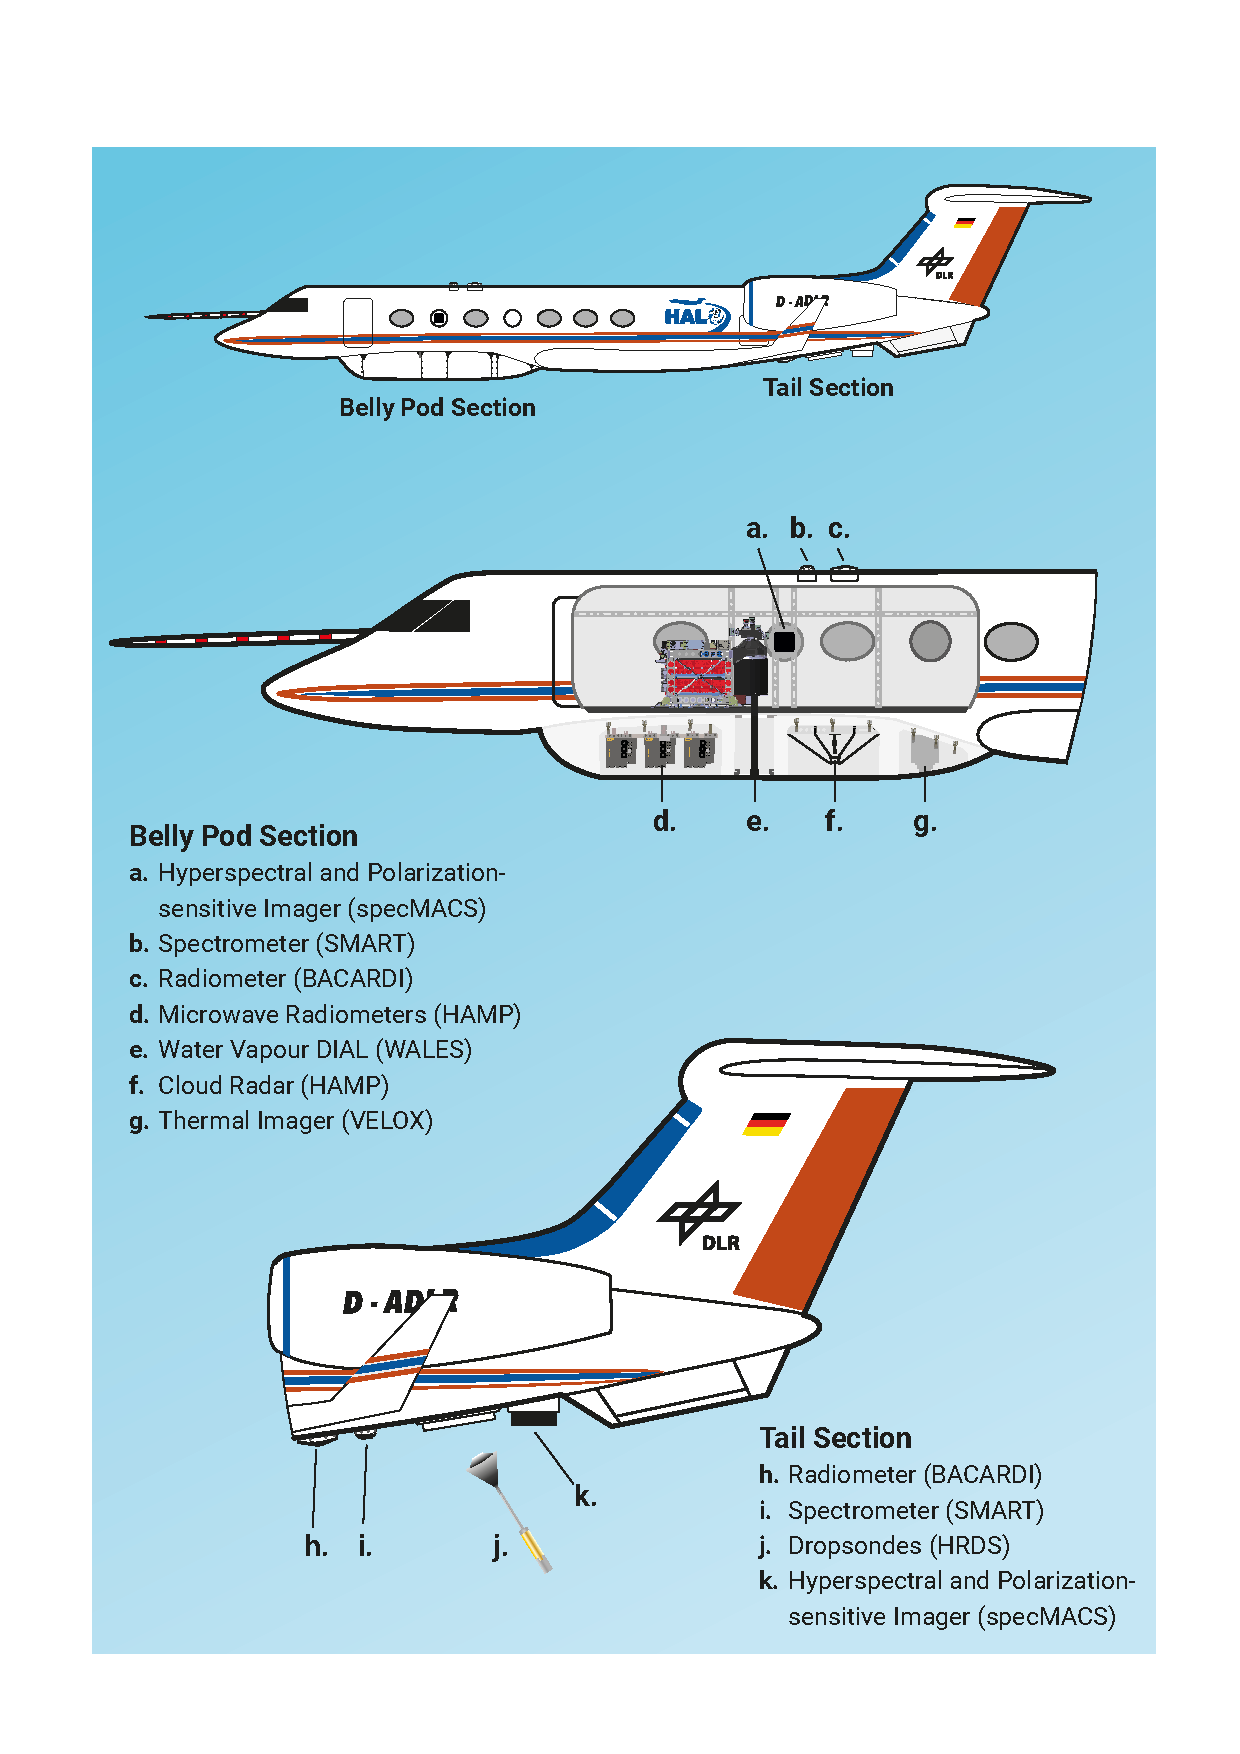
\includegraphics[width=0.75\linewidth]{figures/260330_Halo.pdf}
    \caption{Updated cloud-observatory configuration as used during PERCUSION}
    \label{fig:instrumentation}
\end{figure}

As part of the PERCUSION campaign, a decentralized data distribution strategy was introduced for HALO to ensure scientific datasets are openly accessible, verifiable, and resilient. Moving away from traditional central servers, this approach utilises the InterPlanetary File System (IPFS), which operates on two core principles:

\begin{itemize}
    \item Content Addressing: Datasets are identified by a unique, cryptographically secure Content Identifier (CID) derived from the content itself, acting as an immutable fingerprint. Unlike mutable filenames, any change to the data results in a new CID, guaranteeing strict reproducibility for data analysis.
    \item Peer-to-Peer Networking: Rather than relying on a single server, every computer in the network can both request and serve data. When a user retrieves or pins a dataset locally, they help host it.
\end{itemize}

 The additional option of embedding the CID within citable, permanent DOIs via systems such as DataCite ensures long-term data integrity and scholarly traceability.
 Supported by dedicated infrastructure at DKRZ, GWDG, and partner labs, this distributed architecture ensures high redundancy and eliminates single points of failure.
Following its success during the PERCUSION campaign, this IPFS based way of sharing data was expanded to the entire ORCESTRA campaign. It also underlies the ORCESTRA Data Browser (\url{https://browser.orcestra-campaign.org/}), which dynamically fetches metadata and files directly from IPFS on-demand to ensure the user interface is always synchronized with the underlying data.

\textbf{Missing:}
Updates on SpecMACS, new retrievals?

\section{Campaign Design}

To study the impact and drivers of mesoscale structures in the deep tropics during the ORCESTRA campaign, PERCUSION employed a largely generic flight strategy to sample the Atlantic ITCZ, first in the eastern basin near Sal and subsequently in the western basin near Barbados. As noted in the introduction, PERCUSION also included a third component focused on the calibration and validation of the EarthCARE satellite, which is not discussed here (see \cite{grossPersistentEarthCAREUnderflight2026} for details).

By a generic flight strategy, we mean that flight planning followed a set of objective rules that were applied consistently throughout the campaign. The central idea was to sample the structure of the ITCZ in an ITCZ-based reference frame, i.e. to systematically sample the properties at the edges and in the centre of the ITCZ rather than, for example, targeting the locations of deepest convection. Following \cite{Mapes2018}, the ITCZ was primarily identified through its high column water vapour (CWV) content, with its edges defined either by the 48mm CWV contour or by the strongest CWV gradient. In cases where the CWV field was strongly perturbed, surface wind direction was additionally considered following \cite{windmillerInnerLifeAtlantic2024}.
%The location and width of the Atlantic ITCZ can change by several degrees within the course of days \cite{Chen1982, Frank1983}. 

A summary of rules used for flight planning, together with an example flight, is shown in Fig.~\ref{fig:generic_flight_east}. 
In particular:
\begin{itemize}
\item flights were scheduled on days when an EarthCARE overpass was within operational reach,
\item HALO flew along the EarthCARE ground track, remaining on track for at least twenty minutes before and after the satellite overpass,
%\item dropsonde circles were positioned to sample along the strongest gradients in CWV,
\item when the dominant CWV gradient was oriented north--south: dropsonde circles were placed at the southern and northern edges and in the centre of the ITCZ,
\item when the dominant CWV gradient was oriented east--west (occasionally in the western basin): dropsonde circles were arranged along this gradient
\item whenever possible, HALO operated at the highest feasible altitude, ideally above the tropical high-cloud layer,
\item coordinated observations with other platforms were conducted whenever possible, including overflights of and circles around RV METEOR and the SAFIRE ATR-42.
\end{itemize}

%While deviations from the generic flight strategy are discussed in detail in Section~\ref{sec:implementation}, one systematic modification to the flight plan occurred in the western basin, where the strongest gradients in column water vapour were, at times, oriented primarily in the east-west direction. In these cases, the dropsonde circles were aligned east-west to sample along the strongest column water vapour gradients but without crossing the ITCZ.

\begin{figure}
\centering
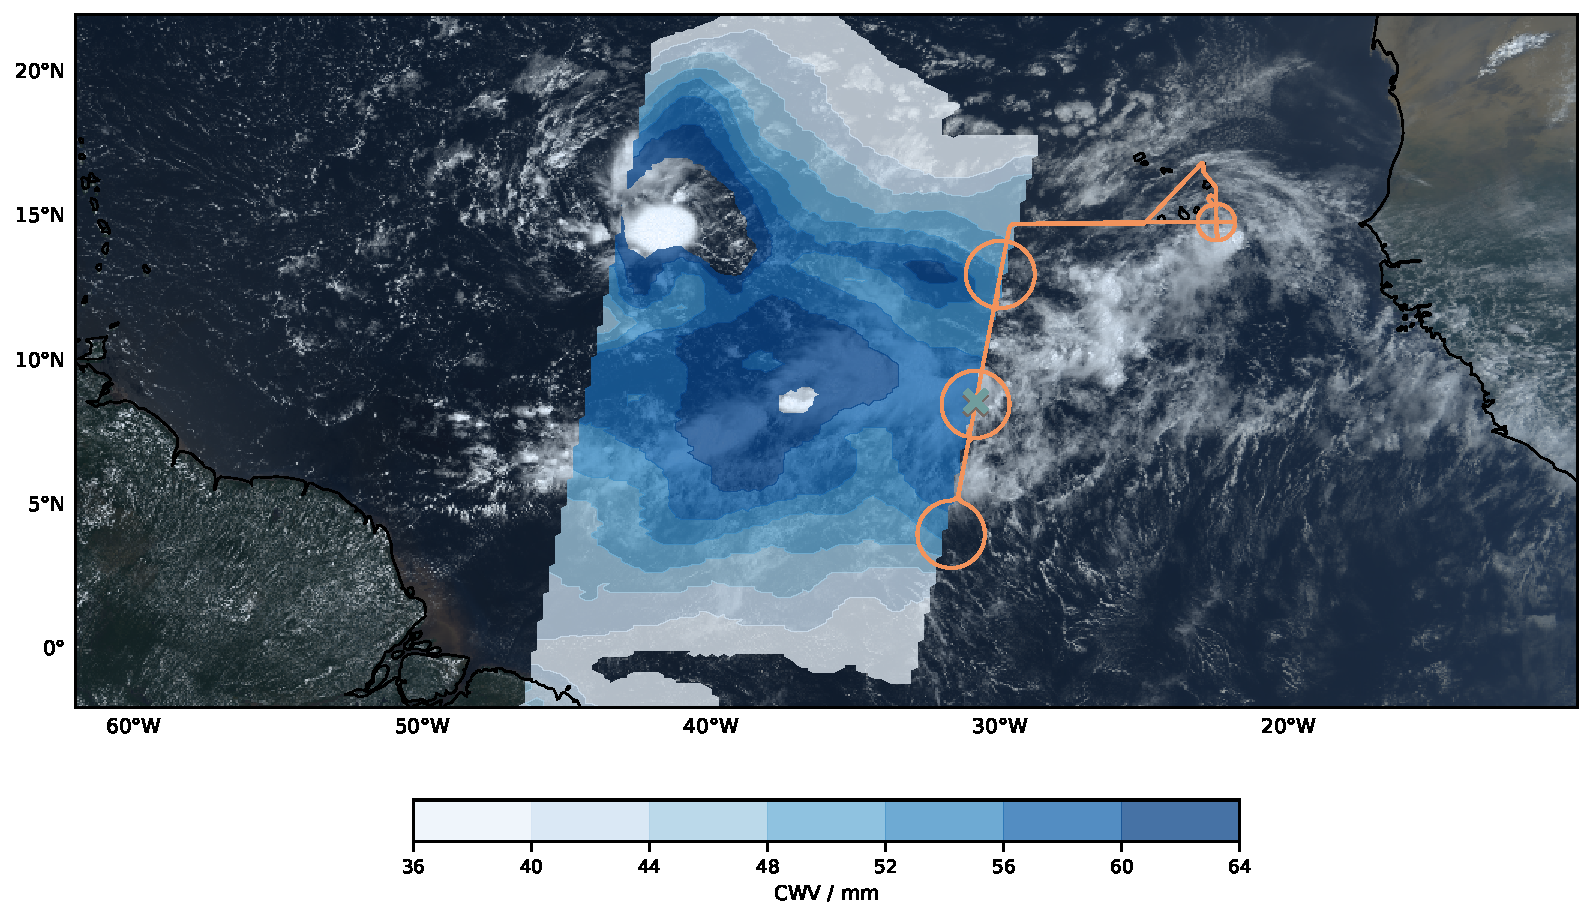
\includegraphics[width=1\linewidth]{figures/HALO-20240903a_flight_track.pdf}
\caption{Example flight (flight ID HALO-20240903a) illustrating the generic flight strategy. The flight track is shown in orange, together with a GOES satellite image in the background (15:20 UTC) and column water vapour measurements from the Advanced Microwave Scanning Radiometer (AMSR).}
\label{fig:generic_flight_east}
\end{figure}

The rationale behind the different elements of the flight strategy was as follows. Flying along the EarthCARE ground track served several purposes. First, as discussed in the introduction, it contributed to the calibration and validation of EarthCARE observations and facilitated the extrapolation of our results to other regions and periods. Second, the repeated back-and-forth pattern along the same track effectively produced three cross-sections of the ITCZ at different times of day: one from EarthCARE and two from HALO. This configuration provides a means of assessing how strongly the mesoscale structure evolves on timescales of a few hours.

The placement of dropsonde circles at the ITCZ edges, or along the dominant CWV gradient, was motivated by the desire to connect the observations as directly as possible to previous studies. In particular, the 48mm CWV contour has been identified as a transition between the deep tropics and the surrounding subsiding regions, while edge intensification refers to precipitation maxima occurring preferentially near this boundary. Vertical velocity measurements in these regions therefore enable a direct comparison with the mechanisms discussed by \cite{Mapes2018}, \cite{masunagaMechanismMaintenanceSharp2020}, and \cite{masunagaEdgeIntensificationEastern2023}.

More generally, defining the ITCZ in terms of CWV provides a natural connection to idealised studies of convective self-aggregation \cite[e.g.][]{Wing2017a}. For example, the moist margins mark the regions where horizontal upgradient moisture transport by a shallow circulation \citep{Muller2012}, if present, is expected to be most efficient.

\section{Implementation and Operational Details}
\label{sec:implementation}

\begin{figure}
    \centering
    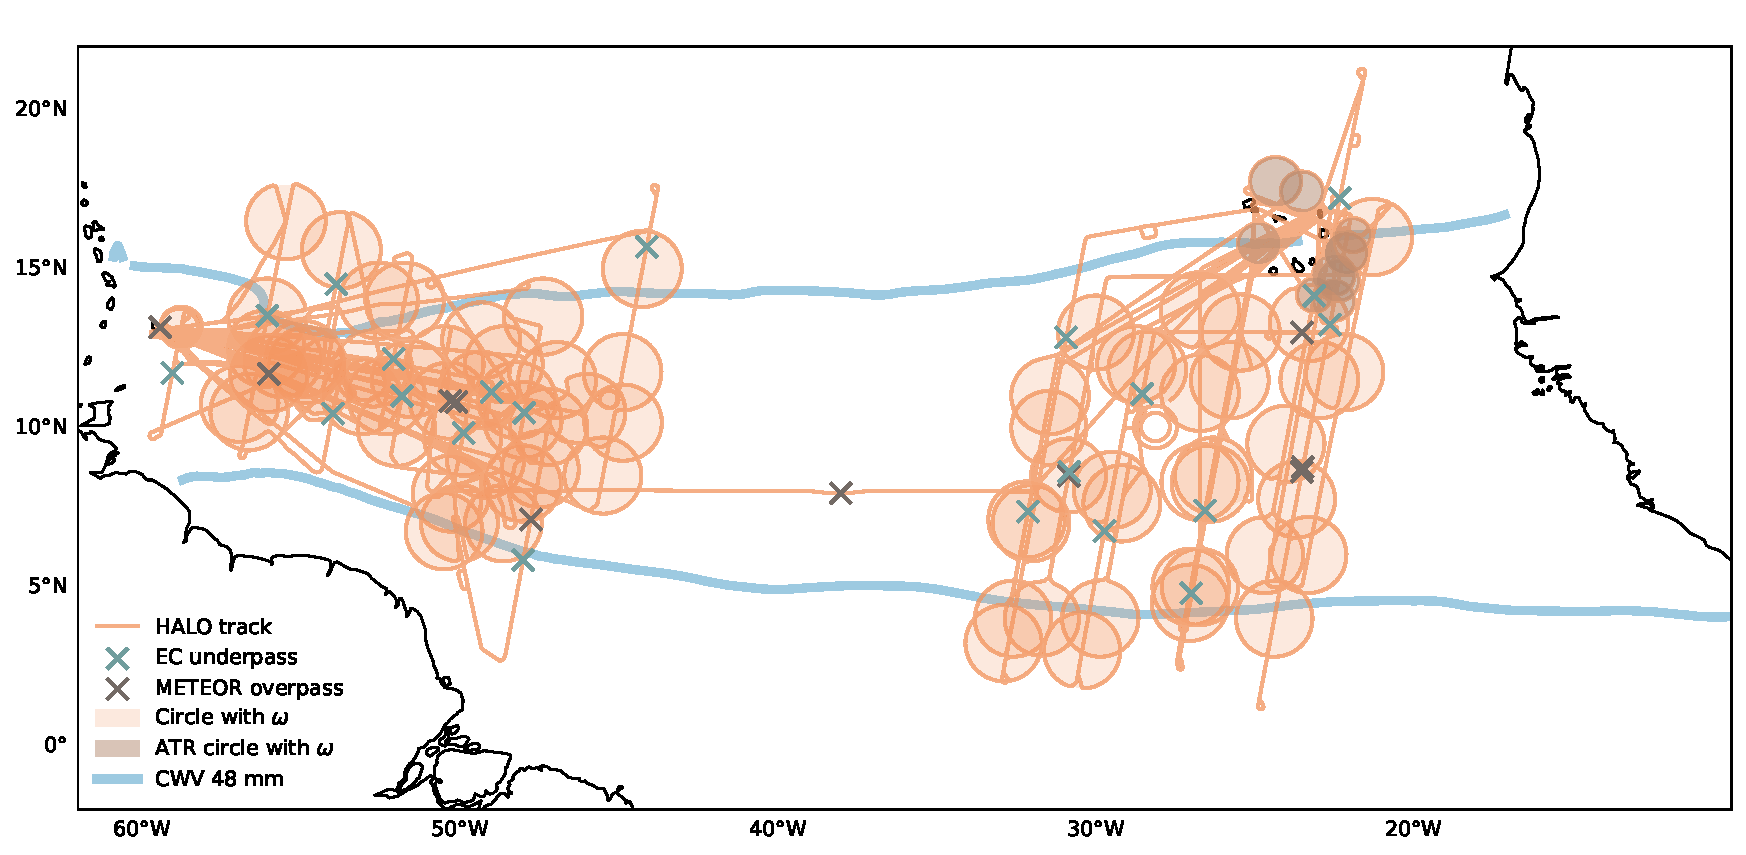
\includegraphics[width=1\linewidth]{figures/flight_overview.pdf}
    \caption{Overview of all research flights conducted during ORCESTRA. Flight tracks are shown in orange, with shaded regions indicating the areas over which vertical velocity profiles were inferred. Circles flown in coordination with the SAFIRE ATR-42 are highlighted in brown. Locations of EarthCARE underpasses are marked by green crosses, while RV METEOR overpasses are indicated by grey crosses. The blue contour shows the mean location of the 48mm column water vapour contour during the campaign period.}
    \label{fig:flight_overview}
\end{figure}

In total, 23 research flights focused on the Atlantic deep tropics were conducted during ORCESTRA and are shown in Fig.~\ref{fig:flight_overview} and summarised in table~\ref{tab:flights}. Of these, 11 flights were conducted in the eastern basin near Sal and 11 in the western basin near Barbados, with one transfer flight connecting Sal and Barbados while carrying out targeted ITCZ measurements.

Of the 23 research flights, 21 included an EarthCARE underpass. The two exceptions 
(\href{https://orcestra-campaign.org/reports/HALO-20240821a.html}{HALO-20240821a} and 
\href{https://orcestra-campaign.org/reports/HALO-20240906a.html}{HALO-20240906a}) were affected by technical issues. In one case, the resulting delay meant that even the closest EarthCARE overpasses on the rescheduled flight day were beyond HALO's operational range. In the other case, the technical issue occurred shortly before takeoff, leaving insufficient time to modify the flight plan in coordination with air traffic control. 
Details of the coordination with EarthCARE and the results of the calibration and validation can be found in \cite{grossPersistentEarthCAREUnderflight2026}.
In addition to coordination with EarthCARE, a defining feature of the HALO operations was the extensive coordination with other platforms. These included 16 overpasses of RV METEOR, 14 coordinated measurement events with the SAFIRE ATR-42, four overpasses of the Cape Verde Atmospheric Observatory (CVAO), two overpasses of the Barbados Cloud Observatory (BCO), and two underpasses of the PACE satellite.

Across all flights, 93 circles were flown (54 counterclockwise, 38 clockwise, and 1 half-half), including 10 coordinated with the SAFIRE ATR-42 and 10 with the RV METEOR. Of these 93 circles, 90 were targeted dropsonde circles designed to calculate area-averaged properties of the three-dimensional wind field. Eighty-seven of these 90 circles contained sufficient dropsonde measurements to infer vertical velocity profiles \citep{gloecknerBEACHBarbadosEastern2025}. One circle could not be sampled because air traffic restrictions prevented dropsonde launches, while two additional circles yielded insufficient data owing to technical issues. As described above, each vertical velocity profile represents the area-averaged vertical motion within an individual circle, indicated by the shading in Fig.~\ref{fig:flight_overview}.

The remaining three circles served other purposes. Two circles during flight 
\href{https://orcestra-campaign.org/reports/HALO-20240818a.html}{HALO-20240818a} were used to encircle an individual convective system identified during the flight. This deviation from the otherwise standard flight pattern was motivated by the testing and development of new specMACS retrievals. %Should we add more?
The remaining circle was flown to gain altitude. 

Throughout the campaign, systematic adaptations to the generic flight strategy were necessary. These included adjustments to enable coordinated measurements with other platforms, responses to weather conditions (e.g.~avoiding severe thunderstorms), airspace restrictions, technical issues, on-board instrument calibration and validation, and targeted manoeuvres to test new retrieval techniques. While these factors led primarily to minor adjustments in the eastern basin, more substantial modifications were required in the western Atlantic. In particular, the combination of stricter airspace restrictions and a more variable CWV field necessitated changes to the sampling strategy. In this region, the strongest CWV gradients were frequently oriented in an east--west direction. In some cases, these gradients were either not clearly identifiable or located too far east to be reachable within the available flight time. Consequently, dropsonde circles in the western Atlantic were often aligned either east--west or in mixed east--west and north--south configurations. Nevertheless, even in cases with predominantly east--west sampling, parts of the flight track remained aligned in the north--south direction in order to maintain sufficient overlap with the EarthCARE ground track for calibration and validation purposes.

\begin{table}
\caption{HALO Flights}
\label{tab:flights}
\begin{tabular}{llllll}

Flight ID & Date & Takeoff & Landing & Coordination & Circles \\
\midrule
\href{https://orcestra-campaign.org/reports/HALO-20240811a.html}{HALO-20240811a} & 08-11 & 11:59 (SAL) & 20:35 (SAL) & ATR, CVAO, EC & 4 \\
\href{https://orcestra-campaign.org/reports/HALO-20240813a.html}{HALO-20240813a} & 08-13 & 14:15 (SAL) & 23:18 (SAL) & ATR, EC & 4 \\
\href{https://orcestra-campaign.org/reports/HALO-20240816a.html}{HALO-20240816a} & 08-16 & 11:35 (SAL) & 20:03 (SAL) & ATR, EC & 4 \\
\href{https://orcestra-campaign.org/reports/HALO-20240818a.html}{HALO-20240818a} & 08-18 & 10:04 (SAL) & 19:03 (SAL) & EC & 5 \\
\href{https://orcestra-campaign.org/reports/HALO-20240821a.html}{HALO-20240821a} & 08-21 & 12:23 (SAL) & 19:52 (SAL) &  & 4 \\
HALO-20240822a & 08-22 & 11:23 (SAL) & 19:40 (SAL) & ATR (2), CVAO, EC & 5 \\
\href{https://orcestra-campaign.org/reports/HALO-20240825a.html}{HALO-20240825a} & 08-25 & 09:14 (SAL) & 18:58 (SAL) & ATR, CVAO, EC & 4 \\
\href{https://orcestra-campaign.org/reports/HALO-20240827a.html}{HALO-20240827a} & 08-27 & 09:59 (SAL) & 19:08 (SAL) & ATR, EC, METEOR (3) & 4 \\
\href{https://orcestra-campaign.org/reports/HALO-20240829a.html}{HALO-20240829a} & 08-29 & 12:20 (SAL) & 20:30 (SAL) & ATR, CVAO, EC & 4 \\
\href{https://orcestra-campaign.org/reports/HALO-20240831a.html}{HALO-20240831a} & 08-31 & 08:51 (SAL) & 17:41 (SAL) & ATR (3), EC, METEOR (2) & 4 \\
\href{https://orcestra-campaign.org/reports/HALO-20240903a.html}{HALO-20240903a} & 09-03 & 11:32 (SAL) & 20:24 (SAL) & ATR (3), EC, METEOR (2) & 4 \\
\href{https://orcestra-campaign.org/reports/HALO-20240906a.html}{HALO-20240906a} & 09-06 & 10:36 (SAL) & 17:56 (BB) & METEOR &   \\
\href{https://orcestra-campaign.org/reports/HALO-20240907a.html}{HALO-20240907a} & 09-07 & 12:49 (BB) & 20:40 (BB) & EC & 3 \\
\href{https://orcestra-campaign.org/reports/HALO-20240909a.html}{HALO-20240909a} & 09-09 & 11:40 (BB) & 20:46 (BB) & EC & 3 \\
\href{https://orcestra-campaign.org/reports/HALO-20240912a.html}{HALO-20240912a} & 09-12 & 11:29 (BB) & 20:05 (BB) & EC & 4 \\
\href{https://orcestra-campaign.org/reports/HALO-20240914a.html}{HALO-20240914a} & 09-14 & 11:29 (BB) & 20:04 (BB) & EC & 4 \\
\href{https://orcestra-campaign.org/reports/HALO-20240916a.html}{HALO-20240916a} & 09-16 & 11:36 (BB) & 20:56 (BB) & EC, METEOR, PACE & 3 \\
\href{https://orcestra-campaign.org/reports/HALO-20240919a.html}{HALO-20240919a} & 09-19 & 11:01 (BB) & 19:56 (BB) & EC, METEOR (2), PACE & 5 \\
\href{https://orcestra-campaign.org/reports/HALO-20240921a.html}{HALO-20240921a} & 09-21 & 11:22 (BB) & 20:07 (BB) & EC, METEOR & 5 \\
\href{https://orcestra-campaign.org/reports/HALO-20240923a.html}{HALO-20240923a} & 09-23 & 11:13 (BB) & 20:06 (BB) & BCO (2), EC, METEOR (4) & 6 \\
\href{https://orcestra-campaign.org/reports/HALO-20240924a.html}{HALO-20240924a} & 09-24 & 15:37 (BB) & 21:46 (BB) & EC & 3 \\
\href{https://orcestra-campaign.org/reports/HALO-20240926a.html}{HALO-20240926a} & 09-26 & 11:42 (BB) & 20:23 (BB) & EC & 5 \\
\href{https://orcestra-campaign.org/reports/HALO-20240928a.html}{HALO-20240928a} & 09-28 & 10:47 (BB) & 20:02 (BB) & EC & 5 \\

\end{tabular}
\end{table}


A summary of all flights is provided in Table~\ref{tab:flights}, which also contains links to the individual flight reports available on the campaign website. The website was actively maintained throughout the campaign and provides extensive additional information for each flight, including the flight plan, movies of the realised flight track overlaid on satellite imagery, descriptions of the overall weather situation, in-flight impressions, instrument status reports, and instrument quicklooks.

\textbf{Missing: Want to say something about the flight segmentation in this section.}

\section{Overview plots}

Overview plots should show that we successfully sampled the mesoscale structure of the ITCZ. 


\subsection{Sampling the ITCZ} 

\subsubsection{Sampling in CWV space}
First: we sampled at the edges and inside the ITCZ as defined by CWV. 

\begin{itemize} 
    \item Figure~\ref{fig:transition}: plot that shows that we placed circles at the edges (48mm) and in the center (larger than 48mm) (HAMP and dropsonde data). 
    \item Out of 89 circles: all dropsondes in 2 circles have CWV below 48 mm and in 42 circles all dropsondes have CWV above 48 mm. This means that we have 45 circles with at least one dropsonde crossing the 48 mm contour.
\end{itemize}

\begin{figure}
\centering
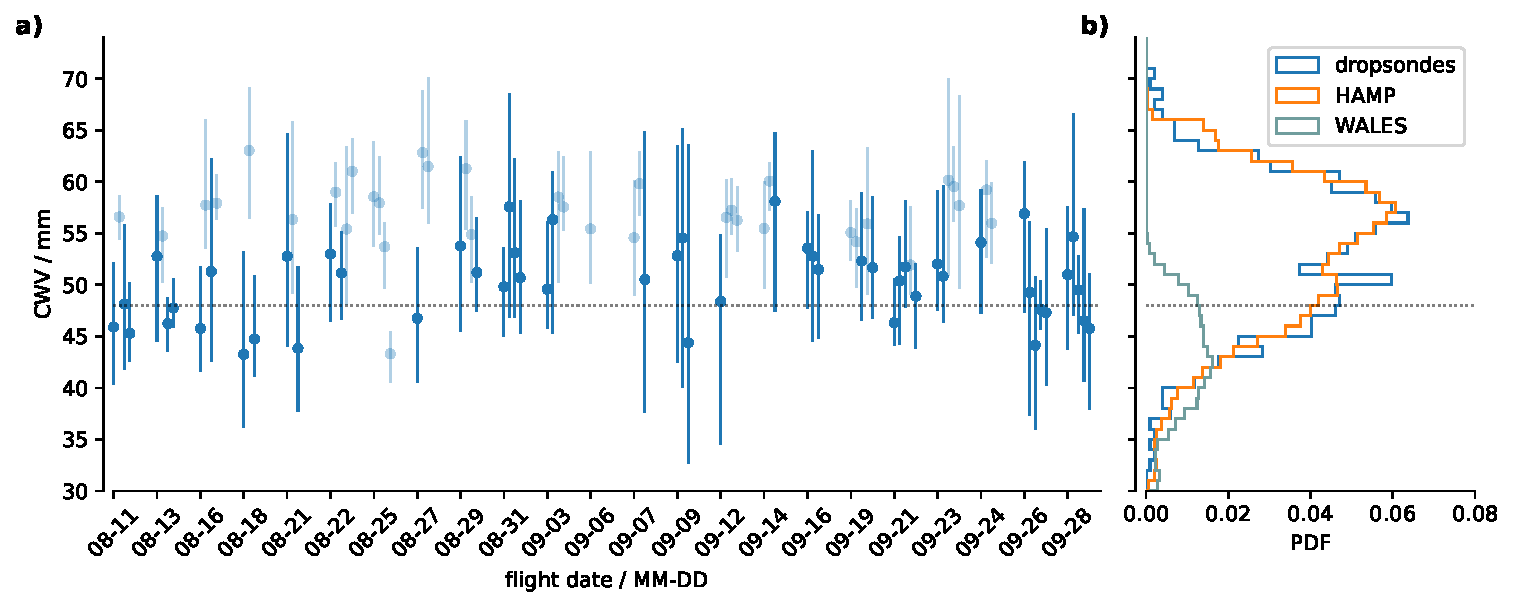
\includegraphics[width=1.0\linewidth]{figures/transition_circles.pdf}
\label{fig:transition}
\caption{ Transition regions and asymmetries. We want to show that our measurement strategy worked and that we have measurements inside and at the (sharp) edges of the ITCZ. \textbf{(top) \textbf{Mean profiles} of water vapour and aerosols from \textbf{WALES} for inside, north, and south of the moist tropics (or define ITCZ differently?)}, (bottom) show how many of the circles actually crossed the 48mm contour (\textbf{dropsondes}) and PDF of CWV caluclated from \textbf{HAMP --- passiv} and \textbf{dropsondes}. \textbf{HAMP IWV still preliminary.}}
\end{figure}

\subsubsection{The ITCZ in CWV space}
\begin{itemize}
    \item Figure~\ref{fig:itcz_cwv}: Show that this successfully captures the transition between subsiding / dry / high OLR and ascending / moist / low OLR region (would be nice to include aerosol or humidity plot from WALES in here!).
\end{itemize}

\begin{figure}
    \centering
    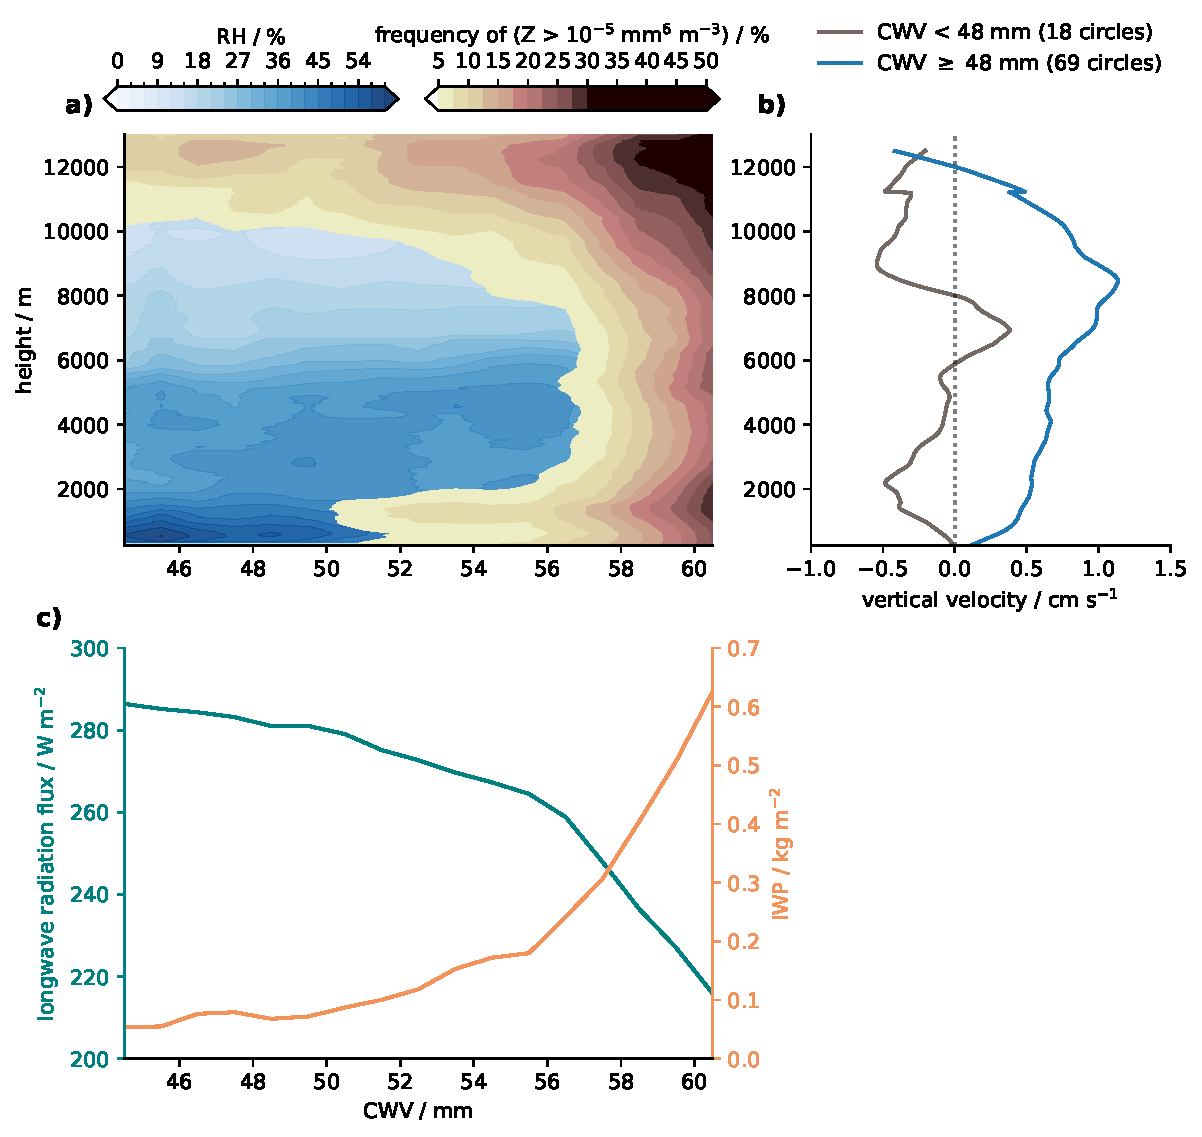
\includegraphics[width=1\linewidth]{figures/itcz_cwv_space.pdf}
    \caption{ITCZ in column water vapour space. (left) cloud occurrence frequency from HAMP radar, relative humidity from WALES, IWP from HAMP passiv and longwave radiation from BACARDI, (right) vertical velocity from dropsondes.}
    \label{fig:itcz_cwv}
\end{figure}

\subsection{Day to day variability of the ITCZ}

Second: the mesoscale structure significantly changed from one day to the next.

\subsubsection{Cloudy ITCZ}
Figure A: with a lot of convective activity (3rd of September)
Note: satellite image is already shown in Fig.~\ref{fig:generic_flight_east}.
Show LAM with dropsondes.
Show one dropsonde circle with ascending motion.
Show measurements from HAMP, VELOX, specMACs (see Fig.~\ref{fig:deep_conv_itcz}).

\begin{figure}
\centering
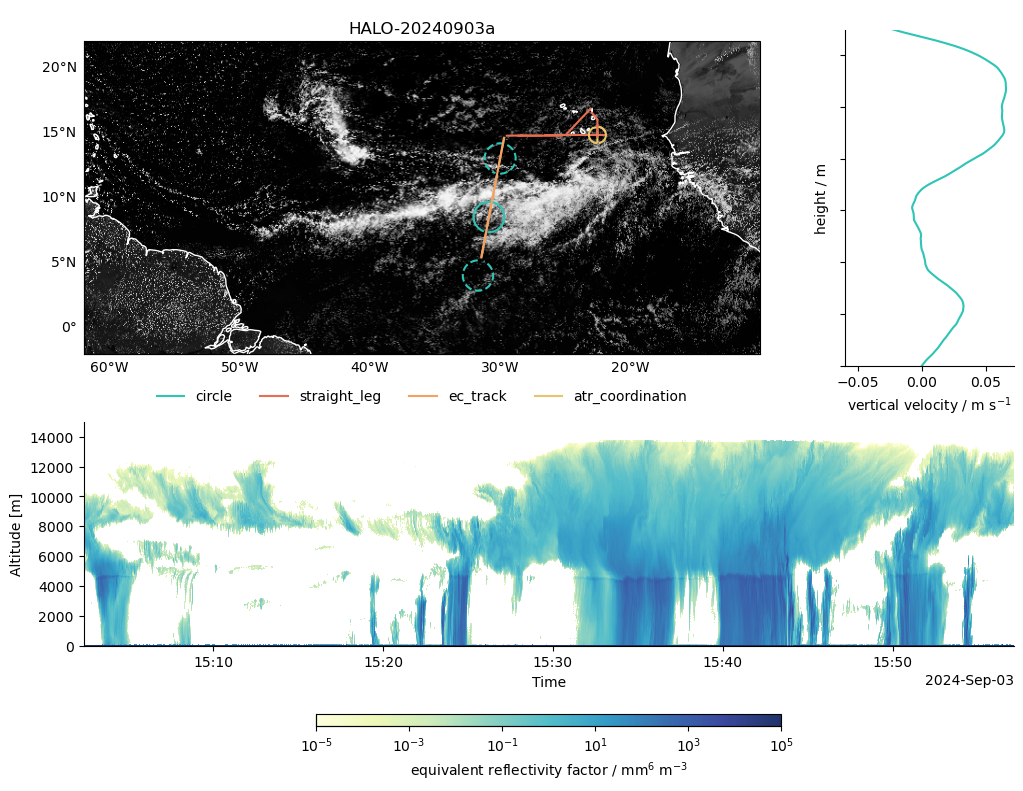
\includegraphics[width=\linewidth]{figures/figures_itcz_deep_convection.png}
\label{fig:deep_conv_itcz}
\caption{ Example of a flight with deep convection in the center of the ITCZ (flight ID HALO-20240903a). Top panel, left: outgoing shortwave radiation from Limited Area Model (LAM) simulations, with elements of the flight as included in the flight segmentation shown in different colours (see legend). Top panel, right: vertical velocity profile for central ITCZ circle. Bottom panel: radar reflectivity from HAMP. \textbf{Include radiation measurements, for example snapshots from VELOX.}}
\end{figure}

\subsubsection{Wind still ITCZ}
Figure B: with little convective activity (but low wind speeds) for the 7th of September. 
Show satellite image (see Fig.~\ref{fig:doldrums_flight_west}).
Show LAM with dropsondes (see Fig.~\ref{fig:doldrums}).
Show one dropsonde circle with subsiding motion.
Show measurements from WALES, specMACs, BACARDI. 

\begin{figure}
\centering
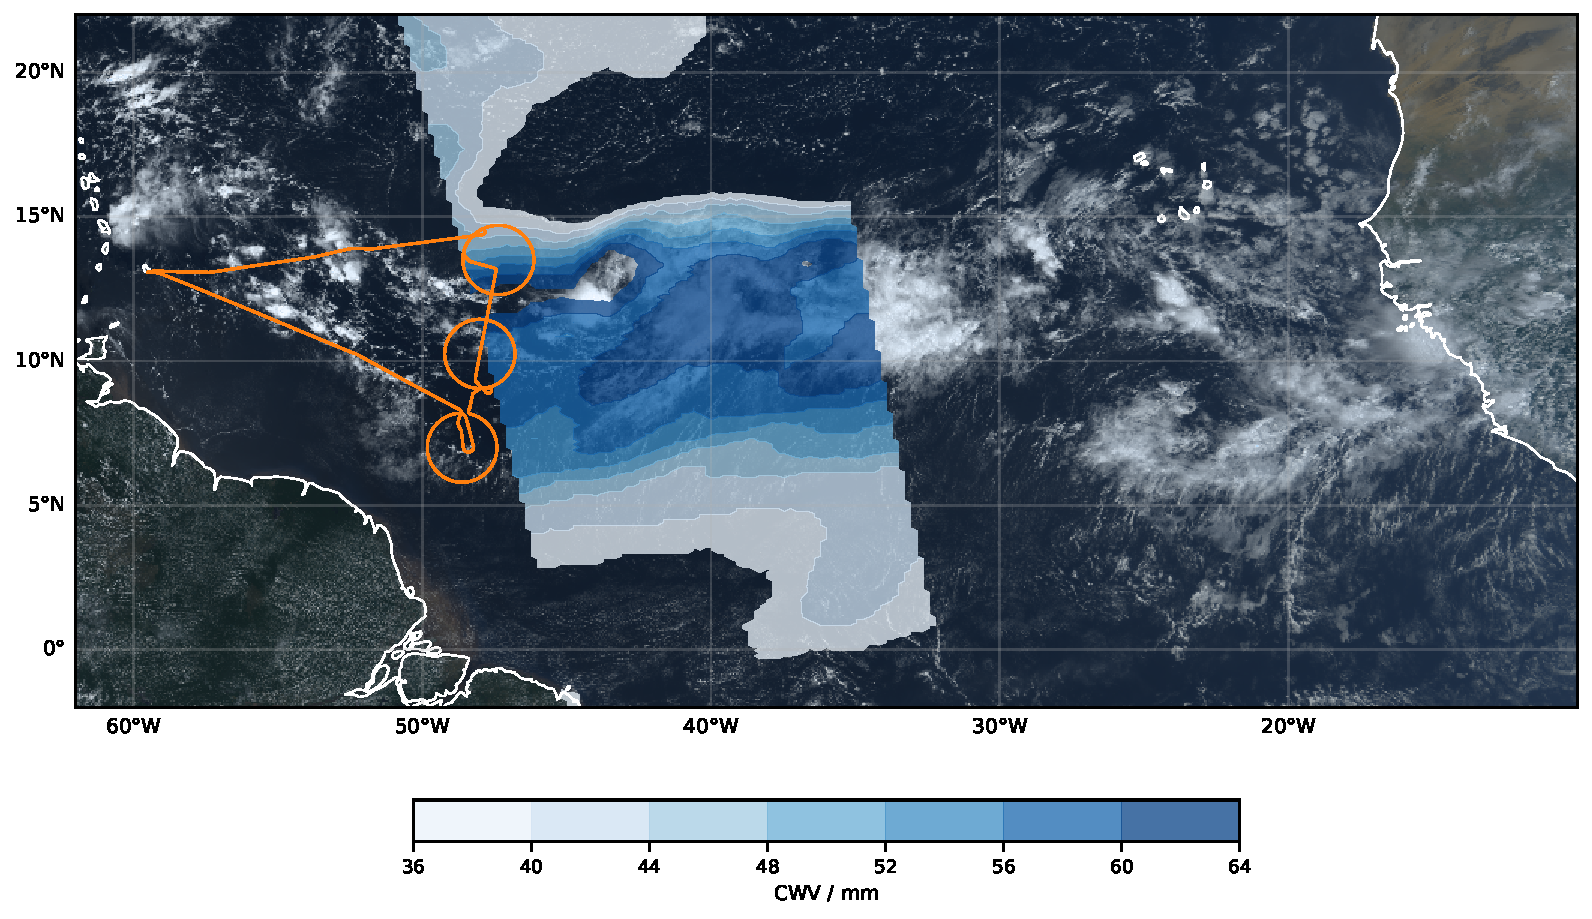
\includegraphics[width=1\linewidth]{figures/HALO-20240907a_flight_track.pdf}
\caption{As in Fig.~\ref{fig:generic_flight_east} but for flight ID HALO-20240907a.}
\label{fig:doldrums_flight_west}
\end{figure}


\begin{figure}
\centering
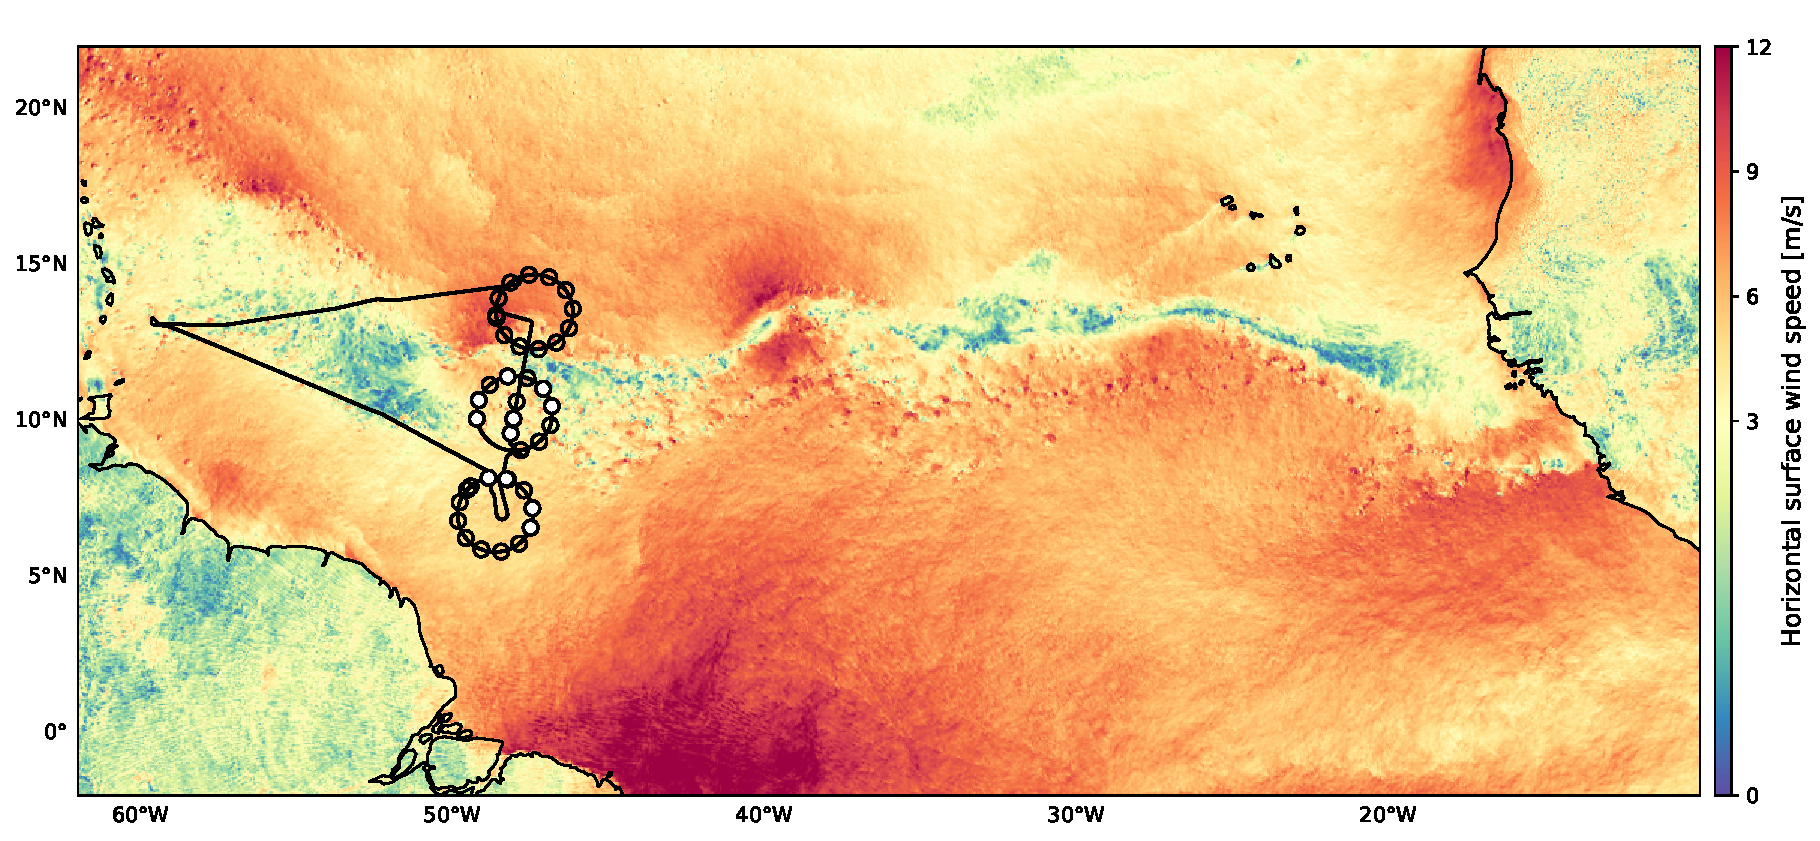
\includegraphics[width=
\linewidth]{figures/doldrums.pdf}
\label{fig:doldrums}
\caption{HALO flight track (black line) and dropsonde locations (black circles) for the flight on the 7th of September 2024. The background shows the horizontal surface wind speed from the limited area model simulations at 16:00 UTC on the same day. Dropsondes with near surface wind speeds less than 3 m/s are filled in white. \textbf{TODO: Would be nice to show some specMACS observations here: can we mark the part of the path with low wind speeds and / or show two images that highlight changes of the specular reflection inside and outside of the doldrums?}}
\end{figure}


% \subsection{Circulation}
% \begin{itemize} 
%     \item tbd
% \end{itemize}

% \begin{figure}
% \centering
% 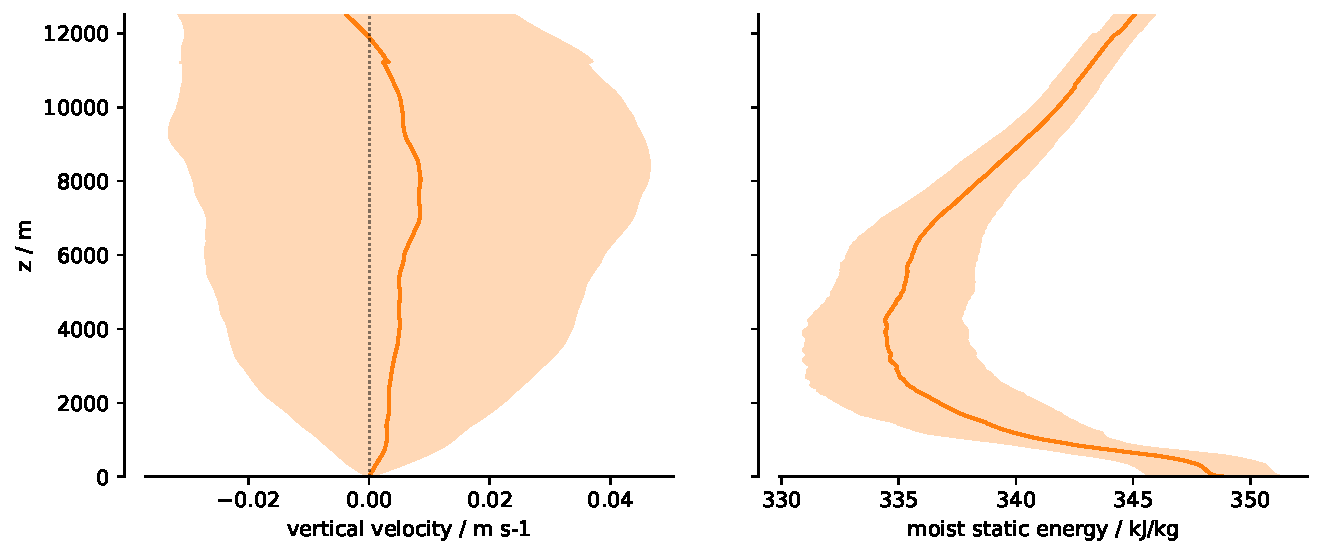
\includegraphics[width=\linewidth]{figures/mse_dynamics.pdf}
% \label{fig:mseDyn}
% \caption{ Overturning circulation and mean moist static energy profile.
% (left) mean area-averaged atmospheric vertical velocity profile from all dropsonde circles. Shaded area shows plus and minus one standard deviation.
% (right) corresponding mean moist static energy profile calculated from the circle averaged temperature and humidity profiles.}
% \end{figure}


\section{Conclusion}

PERCUSION was a measurement campaign with very high resolution data in space and time. 
Disadvantage: limited to a single region and season but our close link to EarthCARE, LAM and GSRM allows us to, in some degree, overcome the disadvantage of an intensive measurement period extrapolate our findings to different regions and seasons.


\section*{Appendix} \begin{itemize} \item Data table with variables and data locations \item Flight segmentation description \end{itemize}

\bibliographystyle{plainnat}
\bibliography{library}


\end{document}

